\textit{1) TX Time}: come mostrato in \textbf{Figura \ref{fig:TXTime_1}}, il tempo medio che le varie antenne di WakeUp passano in TX diminuisce in modo significativo all'aumentare del traffico in rete. Questo risultato giustifica anche quanto è possibile vedere in \textbf{Figura \ref{fig:EnergySpent_1}} in quanto  i vari nodi che ricoprono il ruolo di \textit{receiver}, e che quindi svolgono la funzione di relay per un determinato pacchetto, non inviano più il WakeUp message prima del CTS e in questo modo si vanno a risparmiare \textit{n*m} invii nel caso in cui si hanno \textit{n} potenziali nodi relay e \textit{m} pacchetti data da inviare. In questo caso i miglioramenti sono costantemente tra il 72\% e il 73\%.
\\\\
\textit{2) Energy Consuption}: come mostrato in \textbf{Figura \ref{fig:EnergySpent_1}}, si ha un miglioramento nell'energia complessiva consumata dalla rete alla fine della simulazione. In particolare si ottiene un miglioramento maggiore all'aumentare del traffico in rete, infatti, l'energia consumata diminuisce di circa 7\% nel caso in cui si genera un data packet ogni 50 secondi (circa 65 pacchetti in totale), mentre diminuisce di circa 11\% nel caso in cui si genera un data packet ogni 2 secondi (circa 1700 pacchetti in totale).
\\\\
\textit{3) End-to-End Latency}: come mostrato in \textbf{Figura \ref{fig:Latency_1}}, la latenza è un parametro che ne risente, invece, negativamente. Questo può essere dovuto al fatto che, svegliandosi da solo, il nodo mittente non riesca sempre a ricevere il primo pacchetto CTS per cui deve aspettare il prossimo. Tuttavia, la variante proposta risulta sì più lenta, ma questo ritardo varia da un massimo di 8 millisecondi fino ad un minimo di 6 millisecondi per cui non risulta essere un ritardo particolarmente problematico.
\\\\
\textit{4) Packet Delivery Ratio}: come mostrato in \textbf{Figura \ref{fig:PDR_1}}, il PDR è anch'esso un parametro che risente in modo negativo delle modifiche apportate con autoWakeUp. Dalle simulazioni, così come dal grafico, si evince una perdita di circa lo 0.5\% in più rispetto alla versione base del protocollo nel caso iaTime è 2. Nonostante il PDR più basso, la variante proposta riesce comunque a consegnare sempre almeno il 99.3\% dei pacchetti generati (contro il 99.8\% del base GreenWUP), risultato comunque accettabile nonostante la piccola perdita di qualità.

\begin{figure}[H]
  \begin{subfigure}[t]{0.49\linewidth}
    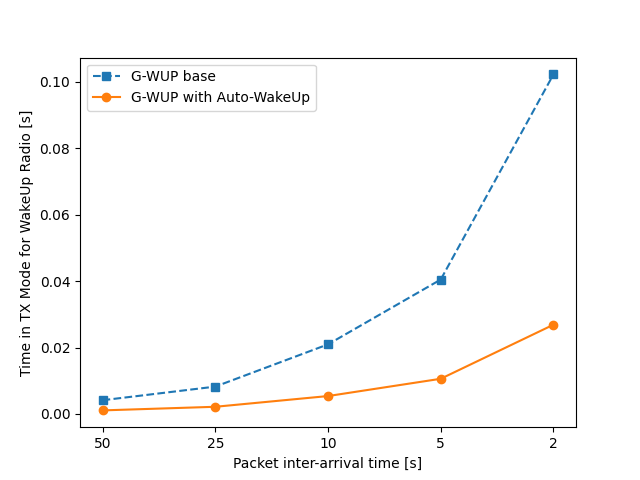
\includegraphics[width=1.1\linewidth]{Contents/Images/graphs/autoWakeUp/tx_time.png}
    \caption{TX Time for the WUR}
    \label{fig:TXTime_1}
  \end{subfigure}
  \begin{subfigure}[t]{0.49\linewidth}
    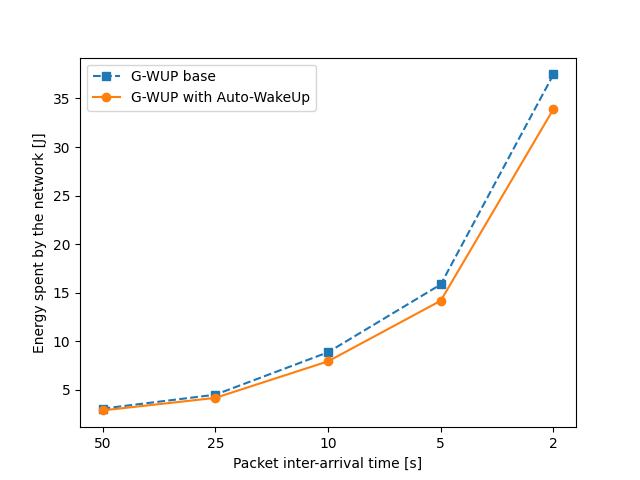
\includegraphics[width=1.1\linewidth]{Contents/Images/graphs/autoWakeUp/energySpent.png}
    \caption{Energy Consuption}
    \label{fig:EnergySpent_1}
  \end{subfigure}
  \begin{subfigure}[t]{0.49\linewidth}
    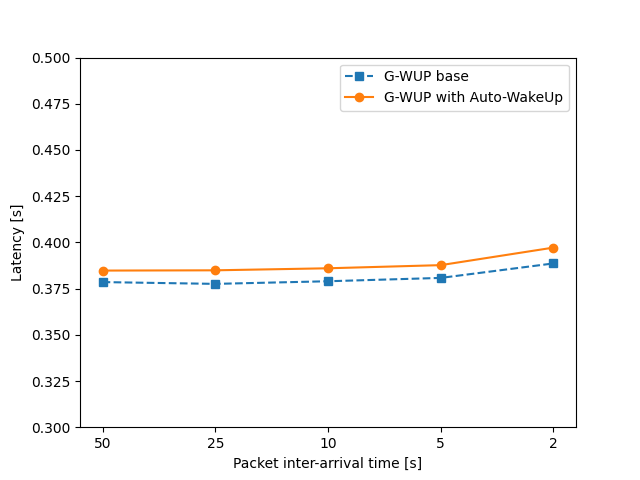
\includegraphics[width=1.1\linewidth]{Contents/Images/graphs/autoWakeUp/latency.png}
    \caption{End-to-End Latency}
    \label{fig:Latency_1}
  \end{subfigure}
  \begin{subfigure}[t]{0.49\linewidth}
    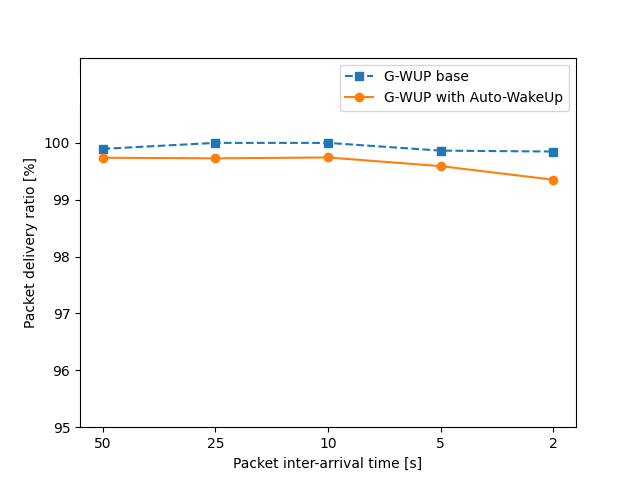
\includegraphics[width=1.1\linewidth]{Contents/Images/graphs/autoWakeUp/pdr.png}
    \caption{Packet Delivery Ratio}
    \label{fig:PDR_1}
  \end{subfigure}
  \caption{Confronto delle prestazioni tra versione base di GreenWUP (blu) e variante proposta (arancio) in termini di energia complessiva consumata, tempo in TX mode della WUR, latenza end-to-end e PDR}
  \label{fig:autoWakeUp}
\end{figure}

In sintesi, il meccanismo introdotto porta ad una ottimizzazione del tempo di trasmissione delle main radio ma non ha benefici significativi sulle
prestazioni end-to-end del sistema.